%%%%%%%%%%%%%%%%%%%%%%%%%%%%%%%%%%%%%%%%%%%%%%%%%%%%%%%%%%%%%%%%%%%%%%%%%%%%%%%%%%%%%
%																					%
%	TRABAJO: Proyecto Integrador													%
%																					%
%		Titulo: 	Desarrollo de IP cores con procesamiento de Redes de Petri 		%
%					Temporales para sistemas multicore en FPGA						%
%																					%
%		Autores:	Juli�n Nonino													%
%					Carlos Renzo Pisetta											%
%		Director:	Orlando Micolini												%
%																					%
%	Parte: Desarrollo																%
%	Capitulo: Implementaci�n en FPGA												%	
%	Archivo: chap_implementacion_fpga.tex											%
%																					%
%%%%%%%%%%%%%%%%%%%%%%%%%%%%%%%%%%%%%%%%%%%%%%%%%%%%%%%%%%%%%%%%%%%%%%%%%%%%%%%%%%%%%

% Path Imagenes: ./desarrollo/implementacion_FPGA/img
% Nombre predeterminado imagenes: implexx
%	xx es el numero de imagen

\lstset
{	language=C,               		% the language of the code
	basicstyle=\footnotesize,       % the size of the fonts that are used for the code
	numbers=left,                   % where to put the line-numbers
	numberstyle=\tiny\color{gray},  % the style that is used for the line-numbers
	stepnumber=1,                   % the step between two line-numbers. If it's 1, each line 
                       				% will be numbered
	numbersep=5pt,                  % how far the line-numbers are from the code
	backgroundcolor=\color{white},  % choose the background color. You must add \usepackage{color}
	showspaces=false,               % show spaces adding particular underscores
	showstringspaces=false,         % underline spaces within strings
	showtabs=false,                 % show tabs within strings adding particular underscores
	frame=none,                 	% adds a frame around the code
	rulecolor=\color{white},        % if not set, the frame-color may be changed on line-breaks within not-black text (e.g. comments (green here))
	tabsize=2,                      % sets default tabsize to 2 spaces
	captionpos=b,                   % sets the caption-position to bottom
	breaklines=true,                % sets automatic line breaking
	breakatwhitespace=false,        % sets if automatic breaks should only happen at whitespace
	%title=\lstname,                % show the filename of files included with \lstinputlisting;
		                            % also try caption instead of title
	keywordstyle=\color{violeta},      % keyword style
  	commentstyle=\color{dkgreen},   % comment style
  	stringstyle=\color{blue},      % string literal style
  	escapeinside={\%*}{*)},         % if you want to add LaTeX within your code
  	morekeywords={*,...},           % if you want to add more keywords to the set
  	deletekeywords={...}            % if you want to delete keywords from the given language
}

\chapter{Implementaci�n en FPGA}
	\label{chap:chap_implementacion_FPGA}

	Para la implementaci�n en una FPGA, se utiliz� el kit de desarrollo de \emph{Digilent Atlys}\footnote{\url{http://www.digilentinc.com/Products/Detail.cfm?NavPath=2,400,836&Prod=ATLYS}} 
	y los programas de la suite \emph{Xilinx ISE Desing Suite}\footnote{\url{http://www.xilinx.com/products/design-tools/ise-design-suite/system-edition.htm}}, 
	\emph{Xilinx Platform Studio} para realizar el dise�o y la implementaci�n del hardware del sistema y 
	\emph{Software Development Kit} para la creaci�n del software que utilizar� el hardware antes mencionado.
	
	En el Ap�ndice \ref{ap:nuevos_proyectos_XPS} se muestra como generar nuevo proyectos en esta herramienta.

	El Ap�ndice \ref{ap:creacion_IP_core} muestra el procedimiento para generar nuevos IP cores. 
	
	Y el Ap�ndice \ref{ap:interrupciones} muestra como agregarles la capacidad de interrumpir.

	En la Figura \ref{fig:diseno01}, donde fue diagramada la arquitectura del sistema, se muestra que el 
	Procesador de Redes de Petri, del cual se ha presentado su dise�o, implementaci�n y prueba en cap�tulos 
	anteriores. 
	Para generar un sistema como el detallado en la Figura \ref{fig:diseno01} se creo un nuevo proyecto en 
	la herramienta \emph{Xilinx Platform Studio}. Luego, se creo un IP core que contenga la l�gica del procesador 
	de Redes de Petri desarrollado y se lo conect� al sistema a trav�s del bus \emph{AXI} \cite{xilinx_axi}.
	
	Luego, se crearon los test necesarios para probar el IP core desarrollado.
	
	En �ste cap�tulo, se mostrar�n los conceptos b�sicos para desarrolar un programa que corra sobre los IP cores
	que ejecutan Redes de Petri y luego, en secciones siguientes, las ejecuciones de dos programas creados para 
	probar el procesador.

	% Programaci�n del sistema
		%%%%%%%%%%%%%%%%%%%%%%%%%%%%%%%%%%%%%%%%%%%%%%%%%%%%%%%%%%%%%%%%%%%%%%%%%%%%%%%%%%%%%
%																					%
%	TRABAJO: Proyecto Integrador													%
%																					%
%		Titulo: 	Desarrollo de IP cores con procesamiento de Redes de Petri 		%
%					Temporales para sistemas multicore en FPGA						%
%																					%
%		Autores:	Juli�n Nonino													%
%					Carlos Renzo Pisetta											%
%		Director:	Orlando Micolini												%
%																					%
%	Parte: Desarrollo																%
%	Capitulo: Dise�o e Implementaci�n en FPGA										%
%	Seccion: Programaci�n del sistema												%	
%	Archivo: programacion.tex														%
%																					%
%%%%%%%%%%%%%%%%%%%%%%%%%%%%%%%%%%%%%%%%%%%%%%%%%%%%%%%%%%%%%%%%%%%%%%%%%%%%%%%%%%%%%

% Path Imagenes: ./desarrollo/implementacion_FPGA/img
% Nombre predeterminado imagenes: implexx
%	xx es el numero de imagen

\section{Programaci�n del sistema}
	\label{sec:programacion}
	
	En el cap�tulo anterior (cap�tulo \ref{chap:chap_diseno_implementacion}) se ha mostrado el
	desarrollo y las caracter�sticas operativas de los IP cores para el procesamiento de Redes
	de Petri. En �sta secci�n se brindar�n las nociones b�sicas para el desarrollo de programas
	que utilicen el IP core. Dado que se trabaja con el procesador MicroBlaze \cite{xilinx_microblaze}
	y el sistema operativo Xilkernel \cite{xilinx_xilkernel}, los c�digos fuentes que se muestran en �ste
	cap�tulo y en los siguientes ser�n para �sta plataforma y en el lenguaje de programaci�n \emph{C}.
	
	\subsection{Manejo de direcciones}
	
		El acceso al IP core se realiza a trave�s de direcciones provistas por el sistema, al momento de
		crear el sistema con el software \emph{Xilinx XPS} \cite{xilinx_edk} es posible determinar manualmente
		el espacio de direcciones para cada IP core o, hacer que la herramienta genere el mapa de direcciones
		autom�ticamente.
		
		Luego, al exportar el proyecto a la herramienta \emph{Xilinx SDK} \footnote{\url{http://www.xilinx.com/tools/sdk.htm}}
		se genera un archivo llamado \emph{xparameters.h}. En dicho archivo, se encuentran las \emph{direcciones base}
		de todos los componentes que conforman el sistema. Despu�s, con la direcci�n base mas un \emph{offset} es posible
		acceder a cada uno de los registros de cada IP core.
		
		Para el IP core con procesamiento de \emph{Redes de Petri con Tiempo}, las direcciones a utilizar son:
		\begin{lstlisting}
//Direcciones para escribir en Petri

Xuint32 *m_marcado_addr    	= (Xuint32 *)(XPAR_TIME_PETRI_AXI_0_BASEADDR);
Xuint32 *m_incidencia_addr 	= (Xuint32 *)(XPAR_TIME_PETRI_AXI_0_BASEADDR + 0x4);
Xuint32 *m_inhibicion_addr	= (Xuint32 *)(XPAR_TIME_PETRI_AXI_0_BASEADDR + 0x8);
Xuint32 *p_cotas_addr 		= (Xuint32 *)(XPAR_TIME_PETRI_AXI_0_BASEADDR + 0xC);
Xuint32 *t_automatica_addr 	= (Xuint32 *)(XPAR_TIME_PETRI_AXI_0_BASEADDR + 0x10);
Xuint32 *load_vector_EFT_addr = (Xuint32 *)(XPAR_TIME_PETRI_AXI_0_BASEADDR + 0x14);
Xuint32 *load_vector_incrementos_tiempo_addr = (Xuint32 *)(XPAR_TIME_PETRI_AXI_0_BASEADDR + 0x18);
Xuint32 *load_vector_LFT_addr	= (Xuint32 *)(XPAR_TIME_PETRI_AXI_0_BASEADDR + 0x1C);
Xuint32 *new_disparo_addr  		= (Xuint32 *)(XPAR_TIME_PETRI_AXI_0_BASEADDR + 0x20);
Xuint32 *sacar_disparo_addr		= (Xuint32 *)(XPAR_TIME_PETRI_AXI_0_BASEADDR + 0x24);
Xuint32 *t_intr_addr			= (Xuint32 *)(XPAR_TIME_PETRI_AXI_0_BASEADDR + 0x28);
Xuint32 *error					= (Xuint32 *)(XPAR_TIME_PETRI_AXI_0_BASEADDR + 0x2C);

//Direcciones para leer en Petri

Xuint32 *leer_disparos_en_espera	= (Xuint32 *)(XPAR_TIME_PETRI_AXI_0_BASEADDR + 0x30);
Xuint32 *leer_disparos_posibles		= (Xuint32 *)(XPAR_TIME_PETRI_AXI_0_BASEADDR + 0x34);
Xuint32 *leer_disparos_ejecutados 	= (Xuint32 *)(XPAR_TIME_PETRI_AXI_0_BASEADDR + 0x38);
Xuint32 *leer_t_num					= (Xuint32 *)(XPAR_TIME_PETRI_AXI_0_BASEADDR + 0x3C);
Xuint32 *red_activa					= (Xuint32 *)(XPAR_TIME_PETRI_AXI_0_BASEADDR + 0x40);
		\end{lstlisting}
		
		Para el caso del IP cora para \emph{Redes de Petri Temporizadas}, las direcciones son:
		\begin{lstlisting}
//	Direcciones para escribir en Petri

Xuint32 *m_marcado_addr    			= (Xuint32 *)(XPAR_TIMED_PETRI_AXI_0_BASEADDR);
Xuint32 *m_incidencia_positiva_addr	= (Xuint32 *)(XPAR_TIMED_PETRI_AXI_0_BASEADDR + 0x4);
Xuint32 *m_incidencia_negativa_addr	= (Xuint32 *)(XPAR_TIMED_PETRI_AXI_0_BASEADDR + 0x8);
Xuint32 *m_inhibicion_addr 			= (Xuint32 *)(XPAR_TIMED_PETRI_AXI_0_BASEADDR + 0xC);
Xuint32 *p_cotas_addr				= (Xuint32 *)(XPAR_TIMED_PETRI_AXI_0_BASEADDR + 0x10);
Xuint32 *t_automatica_addr 			= (Xuint32 *)(XPAR_TIMED_PETRI_AXI_0_BASEADDR + 0x14);
Xuint32 *load_vector_duracion_addr	= (Xuint32 *)(XPAR_TIMED_PETRI_AXI_0_BASEADDR + 0x18);
Xuint32 *load_vector_incrementos_tiempo_addr 	= (Xuint32 *)(XPAR_TIMED_PETRI_AXI_0_BASEADDR + 0x1C);
Xuint32 *t_intr_addr		= (Xuint32 *)(XPAR_TIMED_PETRI_AXI_0_BASEADDR + 0x20);
Xuint32 *error				= (Xuint32 *)(XPAR_TIMED_PETRI_AXI_0_BASEADDR + 0x24);
Xuint32 *new_disparo_addr  	= (Xuint32 *)(XPAR_TIMED_PETRI_AXI_0_BASEADDR + 0x28);
Xuint32 *sacar_disparo_addr	= (Xuint32 *)(XPAR_TIMED_PETRI_AXI_0_BASEADDR + 0x2C);

//	Direcciones para leer en Petri

Xuint32 *leer_disparos_en_espera	= (Xuint32 *)(XPAR_TIMED_PETRI_AXI_0_BASEADDR + 0x34);
Xuint32 *leer_disparos_posibles		= (Xuint32 *)(XPAR_TIMED_PETRI_AXI_0_BASEADDR + 0x38);
Xuint32 *leer_disparos_ejecutados	= (Xuint32 *)(XPAR_TIMED_PETRI_AXI_0_BASEADDR + 0x3C);
Xuint32 *leer_t_num					= (Xuint32 *)(XPAR_TIMED_PETRI_AXI_0_BASEADDR + 0x40);
Xuint32 *red_activa					= (Xuint32 *)(XPAR_TIMED_PETRI_AXI_0_BASEADDR + 0x44);
		\end{lstlisting}
		
	\subsection{Carga de datos}
	
	Para cargar los datos, se debe utilizar la palabra de $32$ bits definida en el cap�tulo \ref{chap:chap_diseno_implementacion}
	en la Figura \ref{fig:diseno07}. Recordando, en dicha palabra, los ocho ($8$) bits m�s significativos representaban la 
	plaza que se deseaba cargar, los siguientes ocho ($8$) bits la transici�n y los �ltimos dieciseis ($16$) bits representaban 
	el dato a cargar. Por ejemplo, para cargar un elemento de la fila $4$, columna $5$ de la matriz de incidencia con el valor 
	$-1$, se debe ingresar el siguiente c�digo:
	\begin{lstlisting}
*(m_incidencia_addr) = 0x0402FFFF;
	\end{lstlisting}
	recordando que \emph{$m_incidencia_addr$} es el par�metro que contiene el valor de la direcci�n para cargar la matriz
	de incidencia como se mostr� en la secci�n anterior.
		
	\subsection{Creaci�n de hilos}
	
		Utilizando el sistema operativo Xilkernel \cite{xilinx_xilkernel}, la forma de crear hilos es la siguiente,
		\begin{lstlisting}
//Funci�n del hilo
void* funcion_hilo();

//Funci�n main
int main()
{
	//Creacion del hilo
		pthread_t hilo;
	
	//Creacion del parametro con atributos para los hilos
		pthread_attr_t attr;
	
	//Inicializacion de atributo para los hilos
		pthread_attr_init (&attr);
	
	//Hacer que los hilos tengan que retornar un valor 
		pthread_attr_setdetachstate(&attr, PTHREAD_CREATE_JOINABLE);
    
    int * valor_de_retorno;
    
    //Poner en funcionamiento el hilo	
    int status = pthread_create(&hilo, &attr, (void*)funcion_hilo, NULL);
    if (status != 0)	{  	xil_printf ("ERROR LANZANDO EL HILO");	}
    
    //Esperar que el hilo termine y tomar su valor de retorno
 		pthread_join(hilo, (void*)&valor_de_retorno);
    return (void*)0;
}

void* funcion_hilo()
{
	int ret = 5;
	pthread_exit((void*)ret);
	return NULL;
}		
		\end{lstlisting}
			
	\subsection{Solicitud de disparo de una transici�n}
		
		Para la solicitud del disparo de una transici�n, se utilizan las direcciones que se han mostrado como
		par�metros algunas secciones antes y la misma palabra de $32$ bits utilizada para cargar los datos.
		\begin{lstlisting}
//Pedir el disparo de la transicion dos (2)
	*(new_disparo_addr) = 0x00020000;
		\end{lstlisting}
		Se utilizas los bits $[23,16]$ para indicar la transici�n que se desea disparar. Luego, el hilo debe esperar
		que el procesador de Redes de Petri resuelva el disparo. �sto, lo puede hacer de tres maneras.
		\begin{itemize}
		  	\item Esperar activamente.
		  	\item Ceder el procesador si el disparo a�n no esta listo.
		  	\item Suspenderse y que cuando el procesador de Redes de Petri resuelva el disparo genere una interrupci�n
		  		lo reactive.
		\end{itemize}
		
		A continuaci�n, se mostrar�n ejemplos de c�digos para los tres casos.
		
		\subsubsection{Espera activa por el disparo}
			
			Cuando se decide que un hilo debe esperar activamente que su disparo este listo, se debe utilziar un c�digo
			similar al siguiente.
			\begin{lstlisting}
//Esperar que T2 se ejecute
	while ( !(*(leer_disparos_ejecutados) & 0x00000004) )
	{	}
			\end{lstlisting}
			Lo que hace el c�digo anterior es acceder al registro del IP core \emph{disparos ejecutados}.
			�ste, es un registro de $32$ donde cada uno de ellos que este en alto indica que la transici�n
			correspondiente a la transici�n con su mismo n�mero ha sido ejecutada.
			
			�sta modalidad, puede ser usada solo en los casos en los cuales se conoce que el hilo puede conseguir que
			su disparo sea ejecutado, por ejemplo, en una situaci�n de simple exclusi�n mutua. 
			
			El problema de la \emph{cena de los fil�sofos}, mostrado en la secc�n \ref{sec:problema_cena_filosofos} es 
			un ejemplo en el cual conviene utilizar �ste m�todo. �sto se debe a que cada \emph{fil�sofo} puede comer 
			todas las veces consecutivas que le sea posible en su franja de tiempo de uso del microprocesador.
			
		\subsubsection{Ceder el paso cuando el disparo a�n no esta ejecutado}
		
			En los casos en los cuales se sabe que el hilo no obtendr� su disparo porque depende de otros disparos
			que deben ser solicitados por otros hilos, conviene que el hilo ceda el procesador cuando comprueba que
			su disparo no est� listo. Ejemplo de �ste caso es el problema del \emph{Escritor/Escritor} mostrado en la
			secci�n \ref{sec:problema_escritor} donde los hilos escriben las variables en turnos ordenados, por lo tanto,
			una vez que uno de los hilos pudo escribir, se sabe que no podr� volver a hacerlo, entonces, debe ceder el
			microprocesador para no ocuparlo innecesariamente.
			
			El c�digo para realizar �sto, es el siguiente:
			\begin{lstlisting}
//Esperar que T2 se ejecute
	while ( !(*(leer_disparos_ejecutados) & 0x00000004) )
	{	yield();	}
			\end{lstlisting}
			
			La sentencia \emph{yield()} fuerza un cambio de contexto liberando el procesador pero, el sistema
			operativo conserva al hilo dentro de su pol�tica de planificaci�n (scheduling).
			
		\subsubsection{Suspensi�n y espera pasiva con interrupciones}
	
			Cuando las transiciones dependen del tiempo, si el tiempo es muy largo, no resulta conveniente que
			el hilo contin�e esperando activamente o cediendo el procesador cada vez que le toca su turno de
			utilzarlo. En dichos casos, conviene que el hilo se suspenda y espere hasta que el procesador de Petri
			ejecute el disparo y genere una interrupci�n para reactivar al hilo.
			
			En �ste caso, la el hilo, despues de solicitar su disparo, debe suspender en un \emph{sem�foro} inicializado
			en $0$ y la funci�n de que atiende las interrupciones lo reactivar�.
	
	\subsection{Extraer un disparo ejecutado}
	
		Luego de que el hilo comprob� que su disparo ha sido ejecutado, antes de proseguir con su ejecuci�n normal,
		debe quitar el disparo de la cola de disparos ya ejecutados. Esto se realiza de la misma manera que cuando
		se solicita un nuevo disparo solo que la direcci�n utilizada para el acceso al IP core es otra. Por ejemplo,
		para extraer el disparo de la transici�n $T2$ una vez que ya se ha ejecutado, el c�digo necesario es el siguiente:
		\begin{lstlisting}
//Pedir el disparo de la transicion dos (2)
	*(sacar_disparo_addr) = 0x00020000;
		\end{lstlisting}
	
	

	% Productor/Consumidor con buffer limitado
		%%%%%%%%%%%%%%%%%%%%%%%%%%%%%%%%%%%%%%%%%%%%%%%%%%%%%%%%%%%%%%%%%%%%%%%%%%%%%%%%%%%%%
%																					%
%	TRABAJO: Proyecto Integrador													%
%																					%
%		Titulo: 	Desarrollo de IP cores con procesamiento de Redes de Petri 		%
%					Temporales para sistemas multicore en FPGA						%
%																					%
%		Autores:	Juli�n Nonino													%
%					Carlos Renzo Pisetta											%
%		Director:	Orlando Micolini												%
%																					%
%	Parte: Desarrollo																%
%	Capitulo: Implementaci�n en FPGA												%
%	Seccion: Productor/Consumidor con buffer limitado								%	
%	Archivo: prod_cons.tex															%
%																					%
%%%%%%%%%%%%%%%%%%%%%%%%%%%%%%%%%%%%%%%%%%%%%%%%%%%%%%%%%%%%%%%%%%%%%%%%%%%%%%%%%%%%%

% Path Imagenes: ./desarrollo/implementacion_FPGA/img
% Nombre predeterminado imagenes: implexx
%	xx es el numero de imagen

\section{Productor/Consumidor con buffer limitado}
	\label{sec:prod_cons}

	En el problema del productor consumidor, existe un buffer, que es compartido por procesos 
	productores que agregan elementos al mismo y elementos consumidores que toman estos elementos.
	
	Se modelar� el problema utilizando Redes de Petri de la siguiente manera.
	
	\begin{figure}[H]
		\centering
		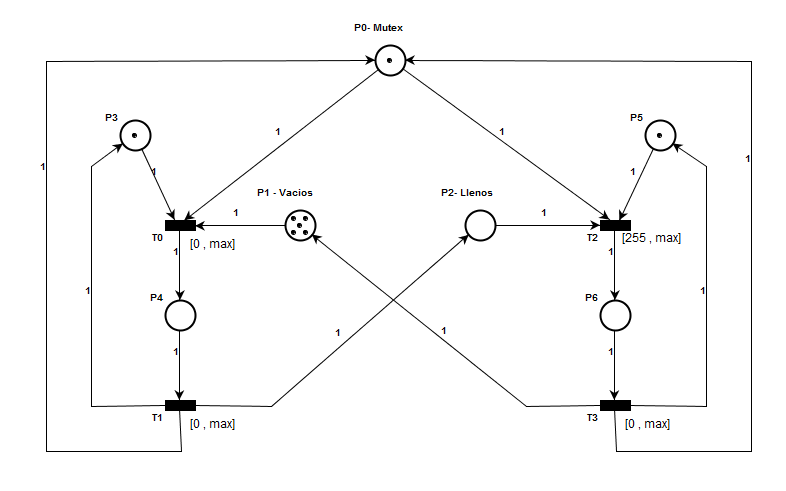
\includegraphics[width=1\linewidth,keepaspectratio]{./desarrollo/implementacion_FPGA/img/imple01}
		\caption{Red de Petri del problema del Productor-Consumidor}
		\label{fig:imple01}
	\end{figure}
	
	Modelando el problema con Redes de Petri, y contando con un procesador capaz de ejecutarlas, 
	es posible validar y verificar las propiedades del modelo y luego, asegurar que la implementaci�n 
	del programa satisface las mismas propiedades del modelo.
	
	\begin{figure}[H]
		\centering
		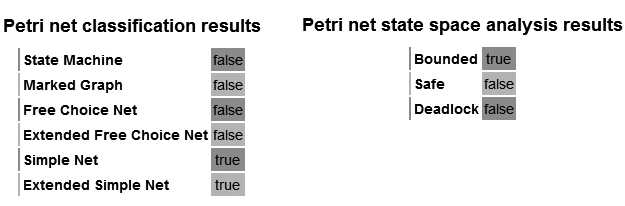
\includegraphics[width=1\linewidth,keepaspectratio]{./desarrollo/implementacion_FPGA/img/imple02}
		\caption{Clasificaci�n y an�lisis del espacio de estados de la Red de Petri}
		\label{fig:imple02}
	\end{figure}
	
	De la Figura \ref{fig:imple02} se observa que la Red de Petri no tiene restricciones en su sintaxis, 
	lo cual, produce que sea clasificada como una Red de Petri simple extendida.
	El an�lisis del espacio de estados de la red que modela el problema del productor consumidor revela 
	que es una red limitada, dado que todas sus plazas tienen l�mites en la cantidad de tokens que pueden 
	albergar pero, no es una red segura. Ya que las plazas relacionadas con el buffer no tienen limites 
	unitarios.
	Adem�s, con este an�lisis, se descubre que la red de Petri NO tiene un estado de deadlock, es decir, 
	siempre esta activa.
	
	\begin{figure}[H]
		\centering
		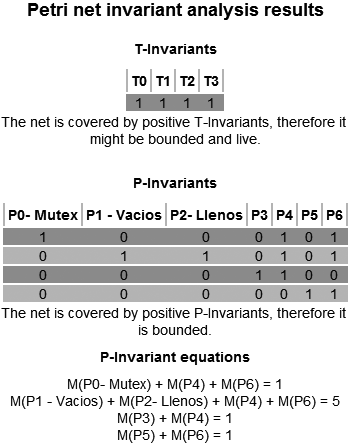
\includegraphics[width=0.5\linewidth,keepaspectratio]{./desarrollo/implementacion_FPGA/img/imple03}
		\caption{An�lisis de invariantes}
		\label{fig:imple03}
	\end{figure}
	
	El an�lisis de invariantes, como se vio en la secci�n \ref{subsec:invariantes}, permite verificar propiedades que se deseaba 
	que el modelo cumpla, como por ejemplo, exclusi�n mutua.

	El an�lisis de los invariantes de transiciones indican que la red esta cubierta por transiciones que generan 
	bucles. En este caso, las cuatro transiciones forman parte de dos bucles que representan al proceso productor 
	y al proceso consumidor. Al existir invariantes de transiciones, se puede decir que la red \emph{podr�a} estar 
	limitada y viva.
	Con la ayuda de los invariantes de plazas, los \emph{t-invariantes} permiten identificar procesos dentro de la 
	Red de Petri.

	Analizando los invariantes de plazas, es posible determinar que la red esta limitada.
	
	El primer invariante de plazas encontrado es:
	\begin{equation}
		M(P0-Mutex) + M(P4) + M(P6) = 1
	\end{equation}
		
	Este invariante, permite asegurar que la propiedad de exclusi�n mutua en el acceso al buffer entre el 
	productor y el consumidor esta garantizada con el modelo que se ha creado. 

	El segundo invariante encontrado es:
	\begin{equation}
		M(P1-Vacios) + M(P2-Llenos) + M(P4) + M(P6) = 5
	\end{equation}

	Esto, demuestra que el l�mite de cinco tokens para el buffer que se ha impuesto, es cumplido en la red.

	Los �ltimos dos invariantes:
	\begin{equation}
		M(P3) + M(P4) = 1
		M(P5) + M(P6) = 1
	\end{equation}

	Junto con el invariantes de transiciones permiten identificar a los procesos productor y consumidor.
	\\

	De esta manera, se ve como se aprovecha el poder de las Redes de Petri para modelar y sistema y para 
	verificar sus propiedades. Luego, como, el procesador de Redes de Petri esta dise�ado para ejecutar 
	estas redes, solo son necesarios la matriz de incidencia y el marcado inicial para generar el software.
	\\
	
	De esta manera, con la herramienta \emph{Xilinx Software Development Kit} se program� la FPGA con un 
	procesador \emph{MicroBlaze} \cite{xilinx_microblaze} conectado al procesador de Redes de Petri y se 
	desarroll� un programa en \emph{C} con dos hilos, uno productor y uno consumidor y utilizan la Red de
	Petri para sincronizar el acceso a la variable compartida. Este programa puede ser consultado en la 
	secci�n \ref{sec:programa_prod_cons}.
	
	Este programa en \emph{C} consta de un hilo principal que realiza la carga de los datos en el procesador 
	de Redes de Petri y da inicio a los hilos productor y consumidor. Los hilos productores y consumidores 
	solo solicitan el disparo de ciertas transiciones.
	Particularmente, el proceso productor solicita el disparo de la transici�n \emph{T0} y espera hasta que 
	�sta se ejecute. Una vez que la transici�n \emph{T0} fue ejecutada, el productor entiende que tiene permiso 
	para trabajar sobre el buffer, lo cual, para el ejemplo implica incrementar un elemento. Luego, solicita el 
	disparo de la transici�n \emph{T1} dejando liberando el control que pose�a sobre el buffer.
	El proceso consumidor se comporta de manera similar solicitando el disparo de la transici�n \emph{T2} para 
	poder trabajar sobre el buffer, quitando un elemento del mismo y disparando la transici�n \emph{T3} para 
	liberarlo.
	\\
	
	Adem�s, se debe mostrar el efecto que producen las restricciones temporales en las transiciones, \emph{T0},
	\emph{T1} y \emph{T3} tienen como intervalo de tiempo $[0;maximo]$. Esto produce que si son solicitadas, 
	al sensibilizarse se disparan.
	La transici�n \emph{T2} tiene como restricci�n temporal el intervalo $[255;maximo]$ esto implica que, desde 
	el instante en el cual es solicitada, deben transcurrir 255 unidades de tiempo luego de que la transici�n se 
	sensibilice para que sea disparada. Esta situaci�n provoca que al comienzo, el hilo productor consiga siempre 
	la exclusi�n mutua pero, cuando el buffer se llena, el productor debe esperar si o si a que el consumidor 
	retire un elemento antes de poder continuar.

	Al ejecutar el programa, se obtiene el siguiente resultado.
	\begin{verbatim}
Comienza la Carga de la Matriz de Incidencia
Termino Carga de la Matriz de Incidencia


Comienza la Carga de la Matriz de Inhibicion
Termino Carga de la Matriz de Inhibicion

Comienza la Carga del vector de Cotas de Plazas
Termino Carga del vector de Cotas de Plazas

Comienza la Carga del vector de Transiciones Automaticas
Termino Carga del vector de Transiciones Automaticas

Comienza la Carga del vector EFT
Termino Carga del vector de EFT

Comienza la Carga del vector de incrementos
Termino Carga del vector de incrementos

Comienza la Carga del vector LFT
Termino Carga del vector de LFT

Comienza la Carga del vector de Marcado Inicial
Termino Carga del vector de Marcado Inicial

Soy el hilo PRODUCTOR - Valor del buffer = 1
Soy el hilo PRODUCTOR - Valor del buffer = 2
Soy el hilo PRODUCTOR - Valor del buffer = 3
Soy el hilo PRODUCTOR - Valor del buffer = 4
Soy el hilo PRODUCTOR - Valor del buffer = 5
Soy el hilo CONSUMIDOR - Valor del buffer = 4
Soy el hilo PRODUCTOR - Valor del buffer = 5
Soy el hilo CONSUMIDOR - Valor del buffer = 4
Soy el hilo PRODUCTOR - Valor del buffer = 5
Soy el hilo CONSUMIDOR - Valor del buffer = 4
Soy el hilo PRODUCTOR - Valor del buffer = 5
Soy el hilo CONSUMIDOR - Valor del buffer = 4
Soy el hilo PRODUCTOR - Valor del buffer = 5
Soy el hilo CONSUMIDOR - Valor del buffer = 4
Soy el hilo PRODUCTOR - Valor del buffer = 5
Soy el hilo CONSUMIDOR - Valor del buffer = 4
	\end{verbatim}
	

	
	% F�brica de mesas
		%%%%%%%%%%%%%%%%%%%%%%%%%%%%%%%%%%%%%%%%%%%%%%%%%%%%%%%%%%%%%%%%%%%%%%%%%%%%%%%%%%%%%
%																					%
%	TRABAJO: Proyecto Integrador													%
%																					%
%		Titulo: 	Desarrollo de IP cores con procesamiento de Redes de Petri 		%
%					Temporales para sistemas multicore en FPGA						%
%																					%
%		Autores:	Juli�n Nonino													%
%					Carlos Renzo Pisetta											%
%		Director:	Orlando Micolini												%
%																					%
%	Parte: Desarrollo																%
%	Capitulo: Implementaci�n en FPGA												%
%	Seccion: F�brica de mesas														%	
%	Archivo: fabrica_mesas.tex														%
%																					%
%%%%%%%%%%%%%%%%%%%%%%%%%%%%%%%%%%%%%%%%%%%%%%%%%%%%%%%%%%%%%%%%%%%%%%%%%%%%%%%%%%%%%

% Path Imagenes: ./desarrollo/implementacion_FPGA/img
% Nombre predeterminado imagenes: implexx
%	xx es el numero de imagen

\section{F�brica de mesas}
	\label{sec:fabrica_mesas}
	
	En este caso, se modelar� de manera sencilla el proceso de fabricaci�n de una mesa.
	Modelando el problema con Redes de Petri, y contando con un procesador capaz de ejecutarlas, 
	podemos validar y verificar las propiedades del modelo y luego, asegurar que la implementaci�n 
	del programa satisface las mismas propiedades del modelo.
	\begin{figure}[H]
		\centering
		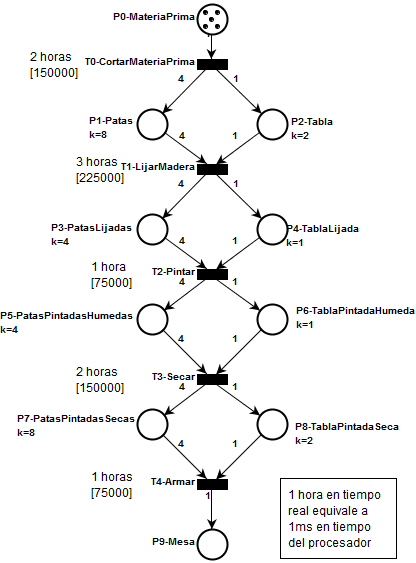
\includegraphics[width=0.75\linewidth,keepaspectratio]{./desarrollo/implementacion_FPGA/img/imple04}
		\caption{Red de Petri que modela una f�brica de mesas}
		\label{fig:imple04}
	\end{figure}
	
	\newpage
	
	Utilizando el software PIPE, se efectuaron ciertos an�lisis sobre la Red de Petri obteniendo 
	los siguientes resultados.
	\begin{figure}[H]
		\centering
		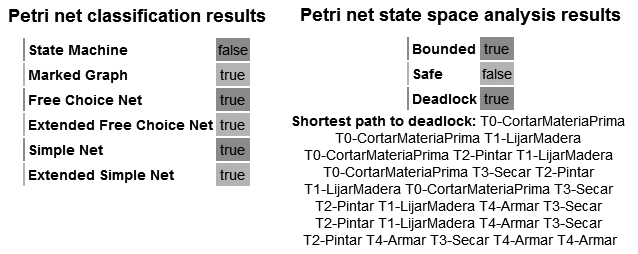
\includegraphics[width=1\linewidth,keepaspectratio]{./desarrollo/implementacion_FPGA/img/imple05}
		\caption{Clasificaci�n y an�lisis del espacio de estados de la Red de Petri}
		\label{fig:imple05}
	\end{figure}
	
	De la Figura \ref{fig:imple05} se observa que la Red de Petri tiene restricciones en su sintaxis, lo cual, 
	produce que sea clasificada como una grafo de marcado. Esto significa, que todas sus plazas tienen un �nico 
	arco de entrada y/o un �nico arco de salida. 
	El an�lisis del espacio de estados de la red que modela el problema planteado, muestra que es una red limitada 
	pero, no es una red segura.
	Adem�s, con este an�lisis, se descubre que la red de Petri tiene un estado de deadlock, la plaza \emph{P9}. 
	Es decir, la Red de Petri, en alg�n momento se detiene, deja de estar activa.
	\\
	
	Para ejecutar la red se instanci� en la FPGA el Procesador de Petri con el agregado de interrupciones para 
	todas las transiciones, de manera que los hilos se duerman para esperar la ejecuci�n de su disparo en vez de 
	preguntar constantemente ya que �stas, no se ejecutar�n hasta que transcurra el tiempo m�nimo en que puede ser 
	disparada la transici�n sensibilizada.
	\\

	Se desarroll� un programa en \emph{C} que carga los valores necesarios en el procesador para ejecutar la red. 
	Luego $5$ hilos encargados cada uno de una actividad distinta piden y retiran el disparo de una transici�n 
	determinada. Una vez terminan la tarea informan de esto mediante consola escribiendo el numero de mesa en el 
	cual estaban trabajando. Este programa, puede encontrarse en la secci�n \ref{sec:programa_fabrica_mesas_petri}.
	
	\newpage

	Al ejecutar el programa, se obtiene el siguiente resultado.
	\begin{verbatim}
Comienza la Carga de la Matriz de Incidencia
Termino Carga de la Matriz de Incidencia 

Comienza la Carga de la Matriz de Inhibicion
Termino Carga de la Matriz de Inhibicion

Comienza la Carga del vector de Cotas de Plazas 
Termino Carga del vector de Cotas de Plazas

Comienza la Carga del vector de Transiciones Automaticas
Termino Carga del vector de Transiciones Automaticas

Comienza la Carga del vector EFT
Termino Carga del vector de EFT

Comienza la Carga del vector de incrementos
Termino Carga del vector de incrementos

Comienza la Carga del vector LFT
Termino Carga del vector de LFT

Comienza la Carga del vector de Marcado Inicial
Termino Carga del vector de Marcado Inicial

Comienza la Carga del vector de Transiciones con Interrupcion
Termino Carga del vector de Transiciones con Interrupcion

Semaforos creados correctamente

Mesa 1: CORTADA
Mesa 2: CORTADA
Mesa 1: LIJADA
Mesa 1: PINTADA
Mesa 1: SECADA
Mesa 3: CORTADA
Mesa 2: LIJADA
Mesa 2: PINTADA
Mesa 2: SECADA
Mesa 1: ARMADA
Mesa 4: CORTADA
Mesa 3: LIJADA
Mesa 3: PINTADA
Mesa 3: SECADA
Mesa 2: ARMADA
Mesa 5: CORTADA
Mesa 4: LIJADA
Mesa 4: PINTADA
Mesa 4: SECADA
Mesa 3: ARMADA
Mesa 5: LIJADA
Mesa 5: PINTADA
Mesa 5: SECADA
Mesa 4: ARMADA
Mesa 5: ARMADA
SE ARMARON 5 MESAS

TODOS LOS HILOS TERMINARON	
	\end{verbatim}
	
